% !TEX root = ../main.tex

\subsection{Gaussian Processes}
\label{sec:opt:GPs}

Informally one can think of a GP \citep{rasmussen2006gaussian} as being a nonparametric 
distribution\footnote{Technically speaking they are a stochastic process not a distribution.} over functions.
Equivalently, one can think of them as being a generalization of a Gaussian distribution
to (uncountably) infinite dimensions.  They are powerful tool for regression, classification~\cite{kuss2005assessing}, 
and feature extraction~\cite{lawrence2004gaussian}.  We focus here on regression as it is generally
the simplest usage and the most relevant to our needs.

A GP is fully specified by a mean function $\mu \colon \vartheta \rightarrow \real$ and covariance function 
$k \colon \vartheta \times \vartheta \rightarrow \real$, the latter of which must be a bounded 
$\left(\text{i.e. }k\left(\theta,\theta'\right)<\infty, \; \forall \theta,\theta' \in \vartheta\right)$ 
and reproducing kernel (we will return to this in depth later).  We can describe a function $f$ as being distributed 
according to a GP:
\begin{align}
\label{eq:GP}
f \left(\theta\right) \sim GP \left(\mu\left(\theta\right), k\left(\theta,\theta'\right)\right)
\end{align}
which by definition means that the functional evaluations realized at any finite number of sample points is distributed according to a multivariate Gaussian. Note that the inputs to $\mu$ and $k$ need not be numeric and as such a GP can be defined over anything for which kernel can be defined.

\begin{figure}[t]
	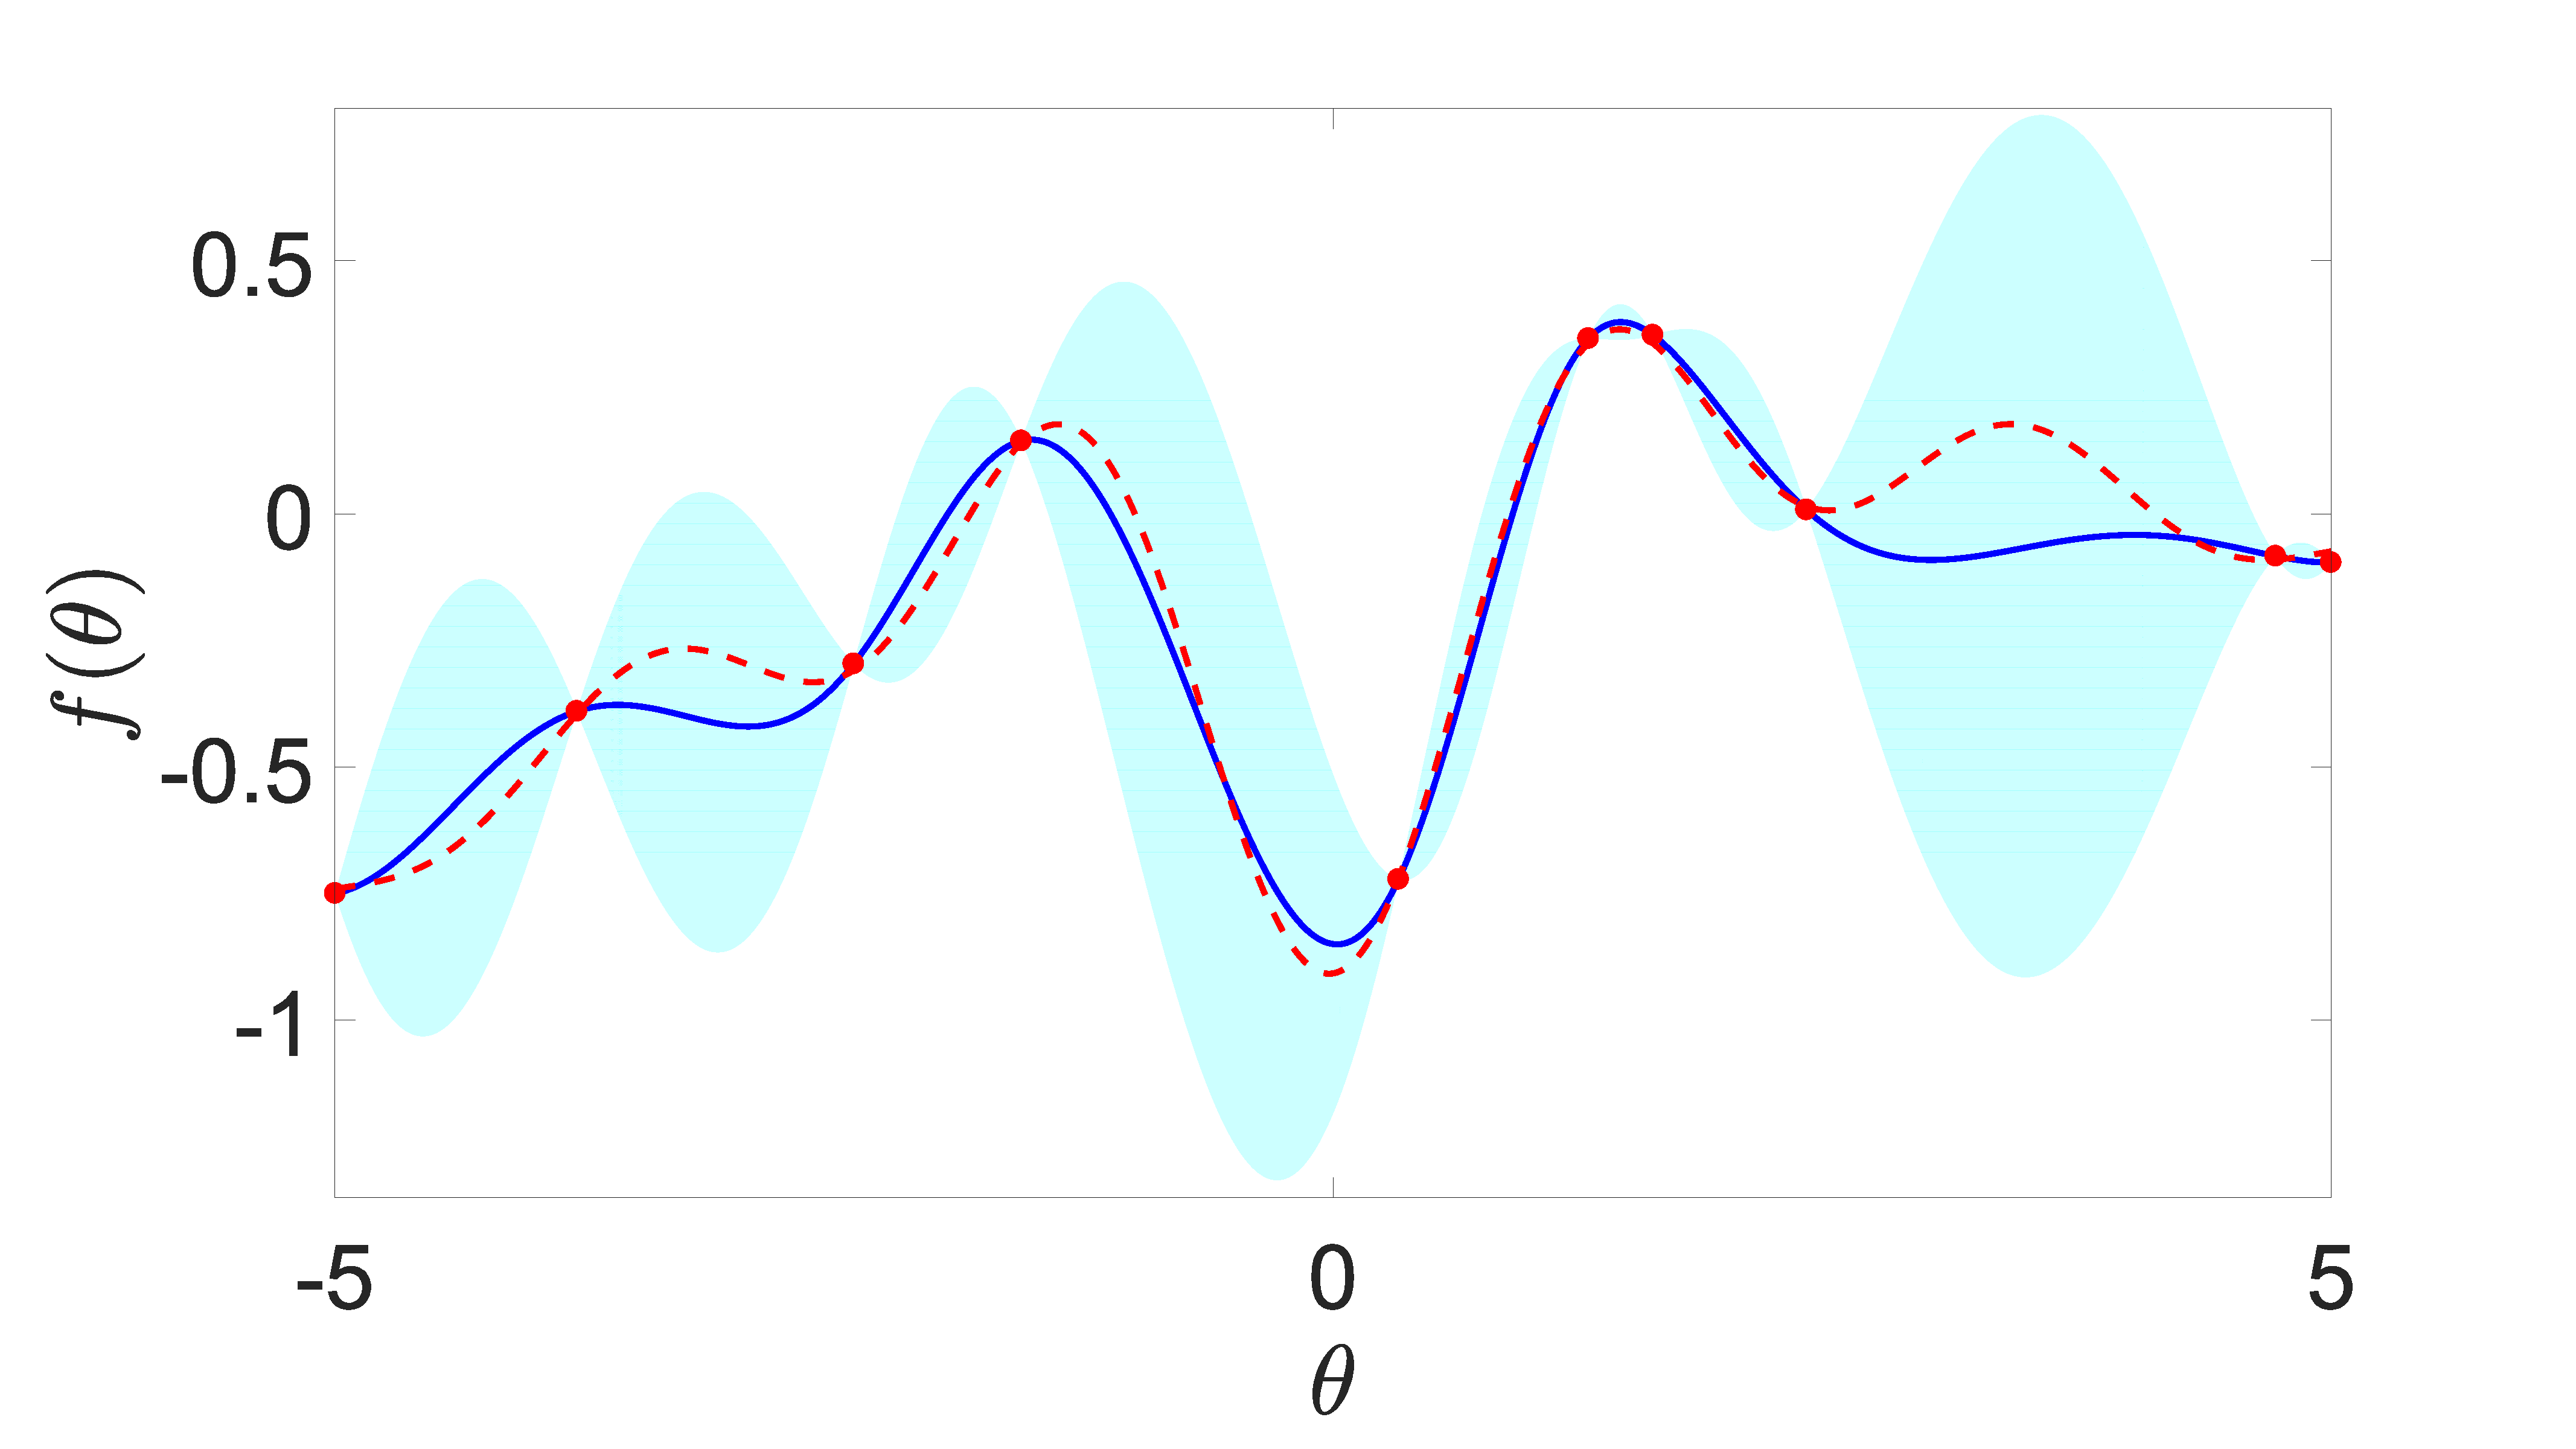
\includegraphics[width=0.49\textwidth]{example_gp}
		~
	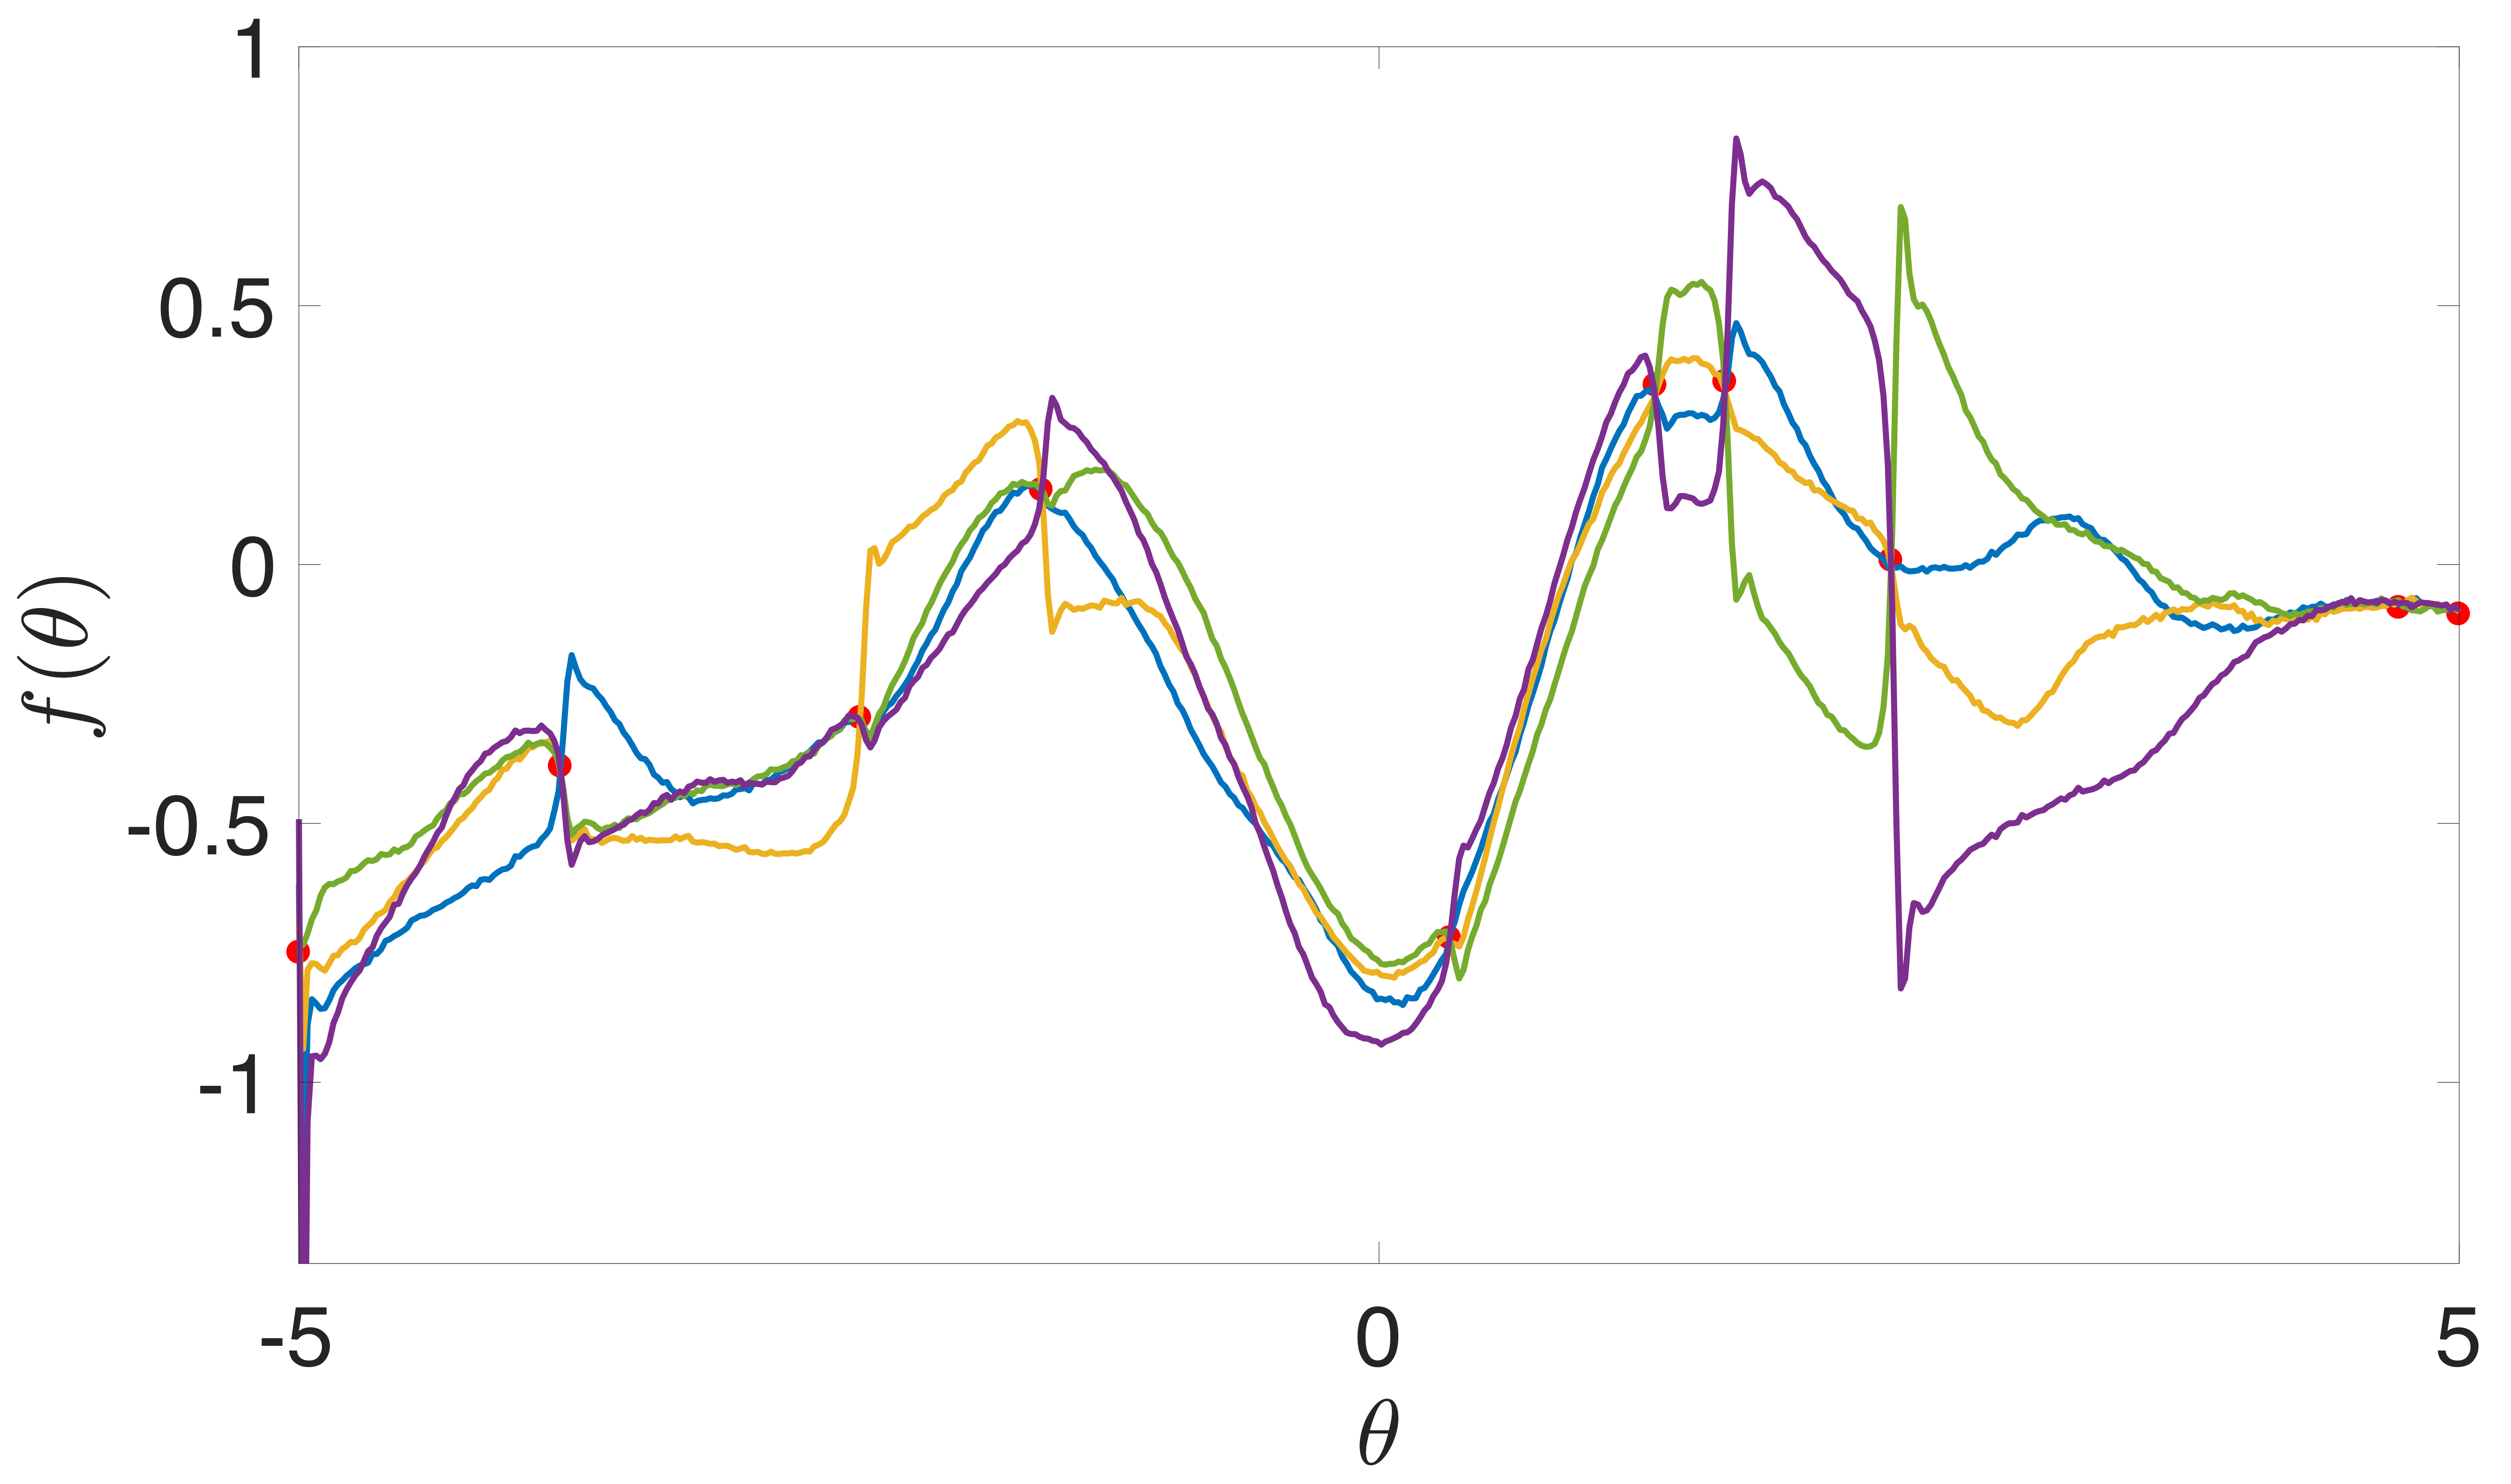
\includegraphics[width=0.49\textwidth]{example_functions}
	\caption{Example GP regression for points shown in left dots.  Shown left is GP where
		the solid dark blue line is the mean of the GP and the light blue shading is the
		mean $\pm2$ standard deviations.  Shown right is 4 example functions drawn
		from the GP which uses a mixture of Mat\'{e}rn-3/2 and Mat\'{e}rn-5/2 kernels
		as per Section~\ref{sec:bopp-for-ml}.\label{fig:opt:example_gp}}
\end{figure}

Figure~\ref{fig:opt:example_gp} shown an example of a GP regression with a small
number of data points.  Here we have placed a GP prior on $f$
\[
f_{\mathrm{prior}} (\theta) \sim \mathrm{GP}\left(\mu_{\text{prior}} (\theta),k_{\text{prior}}\right),
\]
where we take
$\mu_{\text{prior}} (\theta) = 0 \; \forall \theta$ and
\begin{align}
\label{eq:opt:kprior}
\begin{split}
k_{\text{prior}}\left(\theta,\theta'\right) = & \sigma_{3/2}^2 \left(1+\sqrt{3} \; \frac{\theta-\theta'}{\rho_{3/2}}\right)\exp\left(-\sqrt{3} \;\frac{\theta-\theta'}{\rho_{3/2}}\right) +\\&\sigma_{5/2}^2 \left(1+\sqrt{5}\;\frac{\theta-\theta'}{\rho_{5/2}}+\frac{5}{3}\left(\frac{\theta-\theta'}{\rho_{5/2}}\right)^2\right)\exp\left(-\sqrt{5}\;\frac{\theta-\theta'}{\rho_{5/2}}\right)
\end{split}
\end{align}
which corresponds to a combination of a Mat\'{e}rn-3/2 and Mat\'{e}rn-5/2
kernel with hyperparameters $\sigma_{3/2}, \sigma_{5/2}, \rho_{3/2},$ and
$\rho_{5/2}$.  We will return to how to set these later, they are set to
$\sigma_{3/2}=0.05, \sigma_{5/2}=0.78, \rho_{3/2}=0.77,$ and
$\rho_{5/2}=1.42$ in Figure~\ref{fig:opt:example_gp}.

An important property of a GP is that it is conjugate with a Gaussian likelihood.  Consider pairs of input-output data points $\{\hth_j,\hat{w}_j\}_{j=1:m}$, $\hat{W} = \{\hat{w}_j\}_{j=1:m}$, $\hat{\Theta} = \{\hth_j\}_{j=1:m}$ and the separable likelihood function
\begin{align}
\label{eq:GP-lik}
p(\hat{W}| \hat{\Theta}, f) = \prod_{j=1}^{m}p(\hat{w}_j | f(\hth_j)) = \prod_{j=1}^{m}\frac{1}{\sigma_{n}\sqrt{2\pi}} \exp \left(-\frac{\left(\hat{w}_j-f(\hth_j)\right)^2}{2\sigma_n^2}\right)
\end{align}
where $\sigma_n$ is an observation noise. Using a GP prior $f\left(\theta\right)\sim GP(\mu_{\text{prior}}\left(\theta\right),k_{\text{prior}}\left(\theta,\theta\right))$ leads to an analytic GP posterior 
\begin{align}
\label{eq:gpPosterior}
\mu_{post} \left(\theta\right) & = \mu_{\text{prior}}\left(\theta\right) + k_{\text{prior}}\left(\theta,\hat{\Theta} \right) \left[k_{\text{prior}}\left(\hat{\Theta} ,\hat{\Theta}  \right) + \sigma_n^2 I\right]^{-1} \left(\hat{W} -\mu_{\text{prior}}\left(\hat{\Theta} \right)\right) \\
k_{post} \left(\theta,\theta'\right) & = k_{\text{prior}} \left(\theta,\theta'\right) - k_{\text{prior}}\left(\theta,\hat{\Theta} \right) \left[k_{\text{prior}}\left(\hat{\Theta},\hat{\Theta} \right) + \sigma_n^2 I\right]^{-1} k_{\text{prior}}\left(\hat{\Theta} ,\theta'\right)
\end{align}
and Gaussian predictive distribution
\begin{align}
\label{eq:gpPred}
w | \theta, \hat{W}, \hat{\Theta} \sim \mathcal{N} \left(\mu_{post}\left(\theta\right), k_{post} \left(\theta,\theta\right) + \sigma_n^2 I\right)
\end{align}
where we have used the shorthand $k_{\text{prior}}(\hat{\Theta},\hat{\Theta}) = \left[\begin{smallmatrix} k_{\text{prior}}(\hth_1,\hth_1) & k_{\text{prior}}(\hth_1,\hth_2) & \dots\\ k_{\text{prior}}(\hth_2,\hth_1) & k_{\text{prior}}(\hth_2,\hth_2) & \dots \\ \dots & \dots & \dots\end{smallmatrix}\right]$ and similarly for $\mu_{\text{prior}}$, $\mu_{\text{post}}$ and $k_{\text{post}}$.